\documentclass[11pt]{beamer}
\usetheme{Luebeck}
%\usecolortheme{seahorse}
\useinnertheme{rectangles}
\useoutertheme{infolines}
\usepackage{xcolor, natbib}
\usepackage[utf8]{inputenc}
\usepackage{tikz}
\usepackage{tabularx}
\usepackage{lipsum}
\usepackage{amsmath,graphicx,dsfont}
\usepackage{graphicx}
\usetikzlibrary{shapes,backgrounds,arrows,automata,snakes,shadows,positioning, mindmap}
%===================================
\newcommand\pt{\widetilde{p}}
\newcommand{\Ccal}{\mathcal{C}}
\newcommand{\edgeunit}{1.5}
\newcommand{\emphase}[1]{\textcolor{Complement}{#1}}
\newcommand{\bleu}[1]{\textcolor{Framableulight}{#1}}
\newcommand{\pos}[1]{\textcolor{Darkgreen}{#1}}
\newcommand{\nega}[1]{\textcolor{Nicered}{#1}}
\newcommand\independent{\protect\mathpalette{\protect\independenT}{\perp}}\def\independenT#1#2{\mathrel{\rlap{$#1#2$}\mkern2mu{#1#2}}}
\newcommand{\Ncal}{\mathcal{N}}
\tikzset{%
    observed/.style={%
    scale=0.6,circle,draw=Framableulight,transform shape,fill=white,font=\Large}
}
\newcommand{\argmax}{\mathop{\mathrm{argmax}}}   
\newcommand{\backupbegin}{
   \newcounter{framenumberappendix}
   \setcounter{framenumberappendix}{\value{framenumber}}
}
\newcommand{\backupend}{
   \addtocounter{framenumberappendix}{-\value{framenumber}}
   \addtocounter{framenumber}{\value{framenumberappendix}} 
}

\makeatletter
\setbeamertemplate{footline}
{
  \leavevmode%
  \hbox{%
  \begin{beamercolorbox}[wd=.333333\paperwidth,ht=2.25ex,dp=1ex,center]{author in head/foot}%
    \usebeamerfont{author in head/foot}Raphaëlle Momal%~~\beamer@ifempty{\insertshortinstitute}{}{(\insertshortinstitute)}
  \end{beamercolorbox}%
  \begin{beamercolorbox}[wd=.333333\paperwidth,ht=2.25ex,dp=1ex,center]{title in head/foot}%
    \usebeamerfont{title in head/foot}Network inference from count data
  \end{beamercolorbox}%
  \begin{beamercolorbox}[wd=.333333\paperwidth,ht=2.25ex,dp=1ex,right]{date in head/foot}%
    \usebeamerfont{date in head/foot}AgroParisTech seminar\hspace*{2em}
    \insertframenumber{} / \inserttotalframenumber\hspace*{2ex} 
  \end{beamercolorbox}}%
  \vskip0pt%
}
\makeatother
%===================================
\definecolor{Framableu}{RGB}{12,91,122}
\definecolor{Framableulight}{RGB}{18,144,176}
\definecolor{Nicered}{RGB}{176,18,65}
%\definecolor{Nicered}{RGB}{141,14,52}
\definecolor{Lightpink}{RGB}{229,177,218}
\definecolor{Green}{RGB}{144,176,18}
\definecolor{Lightcomplement}{RGB}{235,204,196}
\definecolor{Darkgoldenrod}{RGB}{176,144,18}
\definecolor{Darkomplement}{RGB}{122,43,12}
\definecolor{Complement}{RGB}{176,50,18}
\definecolor{Darkgreen}{RGB}{52,141,14}
%===================================
\setbeamertemplate{itemize items}[square]
\setbeamertemplate{blocks}[shadow=false]
\setbeamertemplate{caption}{\raggedright\insertcaption\par}
%===================================
\setbeamercolor{section in head/foot}{fg=white,bg=Framableu}
\setbeamercolor{subsection in head/foot}{fg=white,bg=Framableulight}
\setbeamercolor{author in head/foot}{bg=Framableu}
\setbeamercolor{item}{fg=Framableulight}
\setbeamercolor*{structure}{bg=Framableulight!20,fg=Framableulight}
\setbeamercolor*{palette secondary}{use=structure,fg=white,bg=structure.fg!75}
\setbeamercolor{section in toc}{fg=Framableu,bg=white}
\setbeamercolor{frametitle}{fg=Framableu!80,bg=white}
\setbeamercolor{block title}{fg=white, bg=Framableulight}  
%===================================
\title{Ecological network reconstruction from count data}

\author{Raphaëlle Momal\\
\tiny{Supervision:  S. Robin$^{{1}}$ and C. Ambroise$^{\inst{2}}$  }}
\institute[]
{
  \inst{1}%
  UMR AgroParisTech/INRA 
  \inst{2}%
  LaMME, Evry
  }
  \date{}
%\date{April 18$^{\text{th}}$, 2019}


%#################################################################

\begin{document}

\begin{frame}
    \titlepage
    \begin{center}
	\includegraphics[width=0.2\linewidth]{agro.PNG}\hspace{0.1cm}
	\includegraphics[width=0.2\linewidth]{logo_inra.jpg}\hspace{0.1cm}
	\includegraphics[width=0.2\linewidth]{lmh.png}\hspace{0.1cm}
	\includegraphics[width=0.08\linewidth]{upsud.jpg}
    
\end{center}
\end{frame}

\section{Motivation}
%====================================================================
%====================================================================

\begin{frame}{Context}

Rising interest in \emphase{jointly analysed }species abundances:
\begin{itemize}
	\item Metagenomics 
	\item Microbiology
	\item Ecology
\end{itemize}
%\pause

\begin{block}{Ecological network}
Tool to better understand species interactions (direct/indirect), eco-systems organizations (hubs?) 
\end{block}\bigskip
%\pause
Allows for resilience analyses, pathogens control, ecosystem comparison, response prediction...
\end{frame}
%====================================================================
%====================================================================


\begin{frame}{Example}
\Large{\bleu{Data:}}\\ \normalsize{}
	\begin{itemize}
	\item \emphase{Species}: bacteria, fungi...
	\item \emphase{Abundances}: read counts from Next-Generation Sequencing technologies (metabarcoding) $\Rightarrow$ \bleu{$n\times p$ matrix $Y$}
	\item \emphase{Covariates}: temperature, water depth...  $\Rightarrow$  \bleu{$n\times d$ matrix $X$}
	\item \emphase{Offsets}: species-specific, sample-specific  $\Rightarrow$ \bleu{$p\times p$ matrix $O$}\bigskip
\end{itemize}
\Large{\bleu{Goal:}}\normalsize{}

	Infer the \emphase{species interaction network} $\widehat{G}$ from count data $Y$, accounting for $X$ and $O$ : $$\widehat{G}=f(Y,X,O)$$

\end{frame}
%====================================================================
%====================================================================
\begin{frame}{Challenges}\large{
	\begin{itemize}
	\item  Statistical network inference \bigskip\bigskip
	\item Count data \bigskip\bigskip
	\item Offsets and covariates
\end{itemize}}
\end{frame}
%====================================================================
%====================================================================

\section{Network inference}
\begin{frame}
\begin{center}
\huge{\bleu{Model}}
\end{center}
\end{frame}
\subsection{General Framework}
%====================================================================
%===================================================================

\begin{frame}{Graphical models: a statistical framework for network inference}
\bleu{Example}:\bigskip
\begin{columns}
\begin{column}{0.3\linewidth}\hspace{0.5cm}
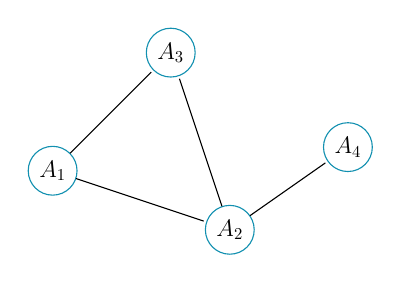
\begin{tikzpicture}	

      \tikzstyle{every edge}=[-,>=stealth',shorten >=1pt,auto,thin,draw]
		\node[observed] (A1) at (0*\edgeunit, 0*\edgeunit) {$A_1$};
		\node[observed] (A2) at (1.5*\edgeunit, -0.5*\edgeunit) {$A_2$};
		\node[observed] (A3) at (1*\edgeunit, 1*\edgeunit) {$A_3$};
		\node[observed] (A4) at (2.5*\edgeunit, 0.2*\edgeunit) {$A_4$};
		\path (A1) edge [] (A2)
        (A1) edge [] (A3)
        (A2) edge [] (A3)
        (A2) edge [] (A4);
	\end{tikzpicture}\\
\end{column}
\begin{column}{0.5\linewidth}
	\begin{itemize}
	\item Connected: all variables are dependant \bigskip
	\item Some are \emphase{conditionally independent} (i.e. indirectly dependant)\\\bigskip
	 $A_4$ is independent from $(A_1, A_3)$ conditionally on $A_2$ \vspace{0.2cm}
\end{itemize}
\end{column}
\end{columns}
%\pause
\begin{center}
    \[ P(A_1, \dots, A_p) \propto \prod_{C \in \Ccal_G} \psi_C(A_C) \]
  where $\Ccal_G =$ set of maximal cliques of $G$.
\end{center}

\end{frame}
%====================================================================
%====================================================================

\section{With count data}
\subsection{Model}

%====================================================================
%====================================================================

\begin{frame}{PLN model \only<3>{+ Graphical model}}
\begin{block}{Poisson log-Normal distribution \citep{AiH89}}
\[
            \left.
                \begin{array}{rl}
               \vspace{0.2cm}    Z_i \textit{ iid } &\sim \mathcal{N}_{d}(0,\Sigma\only<3>{\emphase{_G}})\\
              \vspace{0.2cm}    &(Y_{ij})_j \independent |Z_i\\
                    Y_{ij}|Z_{ij} &\sim \mathcal{P}(e^{\only<2->{\emphase{o_{ij}+x_i^{\text{T}}\Theta_j} +}Z_{ij}}) 
                   
                \end{array}
            \right \} Y \sim \mathcal{P\ell N}(\only<2->{\emphase{O+X^{\text{T}}\Theta }}\only<1>{0}, \Sigma\only<3>{\emphase{_G}})  
            \]
\end{block}

\begin{itemize}
    \item Dependency structure in the Gaussian latent layer
    \item Easy handling of multi-variate data 
  \only<2->{ \item Allow adjustment for covariates and offsets}
  \only<2->{\item Variational estimation algorithm \citep{CMR17}}
\end{itemize}
%\pause

\end{frame}

\section{Proposed methodology}
\subsection{Using trees}
\begin{frame}{Proposed method: PLN + Spanning trees }
Tree structure on PLN latent layer \bigskip
 \begin{block}{EMtree model}
\[
            \left.
                \begin{array}{rl}
                	 \vspace{0.2cm} 						T & \sim \prod_{kl} \emphase{\beta_{kl}} /B\\ 
               \vspace{0.2cm}    Z_i | T \textit{ iid } &\sim \mathcal{N}_{d}(0,\emphase{\Sigma_T})\\
              \vspace{0.2cm}    &(Y_{ij})_j \independent |Z_i| T\\
                    Y_{ij}|Z_{ij},T &\sim \mathcal{P}( e^{o_{ij}+x_i^{\text{T}}\Theta_j+Z_{ij}}) 
                   
                \end{array}
            \right \} Y \sim \mathcal{P\ell N}(O+X^{\text{T}}\Theta, \emphase{\Sigma_T})  
            \]
\end{block}

$$Z_i \sim \sum_{T\in \mathcal{T}} P(T) \mathcal{N}(0,\Sigma_T)$$
  \end{frame}

%====================================================================
%====================================================================
\begin{frame}{Tree structured data}
\begin{columns}
 \begin{column}{0.7\linewidth}
 \begin{itemize}
    \item Decomposable law for a tree (\cite{kirshner})\\
    $$ P(T) = \prod_{jk} \beta_{jk} / B $$
    \item Likelihood \emphase{factorizes on nodes and edges} \citep{ChowLiu}:
    \end{itemize}
 \end{column}
 \begin{column}{0.3\linewidth}
 \begin{center}
     \includegraphics[width=3cm]{arbredependance.PNG}   
    \end{center}
 \end{column}
\end{columns}

\[P(Z_i|T) =\prod_{j=1}^d P(Z_{ij})\prod_{k,l \in T}\psi_{kl}(Z_i) \hspace{0.3cm},\]

Where \[ \psi_{kl}(Z_i) = \frac{P(Z_{ik},Z_{il})}{P(Z_{ik})\times P(Z_{il})}.\]\\

\end{frame}

\begin{frame}{Why Spanning trees}

 \begin{description}

\item[Sparse structures: ]\begin{itemize}
\item[]
\end{itemize}
\emphase{$\text{\#} \mathcal{G}_p = 2^{\frac{p(p-1)}{2}}$}  reduced to  \emphase{$\text{\#} \mathcal{T}_p = p^{(p-2)}$}\bigskip\bigskip 
%\pause
	\item[Suitable algebraic tool: ]\begin{itemize}
\item[]
\end{itemize}
Matrix tree theorem \citep{matrixtree}
$$\emphase{ \sum_{T\in \mathcal{T}}}\prod_{(k,l) \in T} \psi_{k,l}(Y) = \det(L_{\psi(Y)})  \rightarrow \emphase{\Theta (p^3)}$$

\end{description}
	
%\vskip 
\center{
\textbf{Approach}: infer the network by \emphase{averaging spanning trees}}
	
 
\end{frame}
%====================================================================
%====================================================================

\begin{frame}{Tree averaging} 
\begin{center}
    

%\begin{tabular}{p{\linewidth}}
%\begin{tabularx}{\linewidth}{ccccl}
 \begin{tabular}{ccccl}
   \begin{tabular}{c}
	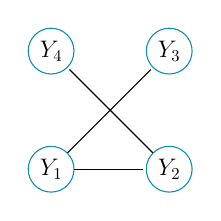
\begin{tikzpicture}
		
      \tikzstyle{every edge}=[-,>=stealth',shorten >=1pt,auto,thin,draw]
    
		\node[observed] (Z1) at (0*\edgeunit, 0*\edgeunit) {$Y_1$};
		\node[observed] (Z2) at (1*\edgeunit, 0*\edgeunit) {$Y_2$};
		\node[observed] (Z3) at (1*\edgeunit, 1*\edgeunit) {$Y_3$};
		\node[observed] (Z4) at (0*\edgeunit, 1*\edgeunit) {$Y_4$};
		\path (Z1) edge [] (Z2)
        (Z1) edge [] (Z3)
        (Z2) edge [] (Z4);
   
	\end{tikzpicture}\\
	\footnotesize{$P\{T = T_1 | Y\}$}
	   \end{tabular}
	   & 
	   \hspace{-.05\textwidth}% \pause
	   \begin{tabular}{c}
		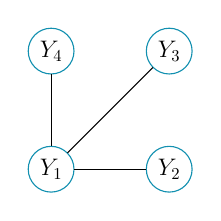
\begin{tikzpicture}
		\tikzstyle{every observed}=[draw=none,text=black,scale=0.5,
      transform shape,circular drop shadow] 
		\node[observed] (Z1) at (0*\edgeunit, 0*\edgeunit) {$Y_1$};
		\node[observed] (Z2) at (1*\edgeunit, 0*\edgeunit) {$Y_2$};
		\node[observed] (Z3) at (1*\edgeunit, 1*\edgeunit) {$Y_3$};
		\node[observed] (Z4) at (0*\edgeunit, 1*\edgeunit) {$Y_4$};
		
		\path (Z1) edge [] (Z2)
        (Z1) edge [] (Z3)
        (Z1) edge [] (Z4);
		\end{tikzpicture} \\
		\footnotesize{$P\{T = T_2 | Y\}$}
	   \end{tabular}
	   &
	   \hspace{-.05\textwidth} %\pause
	   \begin{tabular}{c}
		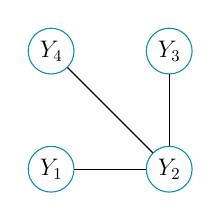
\begin{tikzpicture}
		\tikzstyle{every observed}=[draw=none,text=black,scale=0.5,
      transform shape,circular drop shadow] 
		\node[observed] (Z1) at (0*\edgeunit, 0*\edgeunit) {$Y_1$};
		\node[observed] (Z2) at (1*\edgeunit, 0*\edgeunit) {$Y_2$};
		\node[observed] (Z3) at (1*\edgeunit, 1*\edgeunit) {$Y_3$};
		\node[observed] (Z4) at (0*\edgeunit, 1*\edgeunit) {$Y_4$};
		
		\path (Z1) edge [] (Z2)
        (Z2) edge [] (Z3)
        (Z2) edge [] (Z4); 
		\end{tikzpicture}\\
		\footnotesize{$P\{T = T_3 | Y\}$}
	   \end{tabular}
	   &
	   \hspace{-.05\textwidth}% \pause
	   \begin{tabular}{c}
		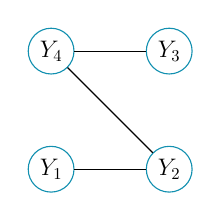
\begin{tikzpicture}
		\tikzstyle{every observed}=[draw=none,text=black,scale=0.5,
      transform shape,circular drop shadow] 
		\node[observed] (Z1) at (0*\edgeunit, 0*\edgeunit) {$Y_1$};
		\node[observed] (Z2) at (1*\edgeunit, 0*\edgeunit) {$Y_2$};
		\node[observed] (Z3) at (1*\edgeunit, 1*\edgeunit) {$Y_3$};
		\node[observed] (Z4) at (0*\edgeunit, 1*\edgeunit) {$Y_4$};
		 
		\path (Z1) edge [] (Z2)
        (Z3) edge [] (Z4)
        (Z2) edge [] (Z4);
		\end{tikzpicture} \\
		\footnotesize{$P\{T = T_4 | Y\}$}
	   \end{tabular}
	   & \hspace{-.06\textwidth} 
	   \huge{\emphase{...}}\normalsize   \\ \\
	   \\% \pause
	   \begin{tabular}{l}
		Compute edge\\
		probabilities:
	   \end{tabular}
	   &
	   \hspace{-.05\textwidth}
	   \begin{tabular}{c}
		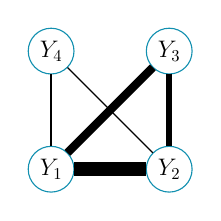
\begin{tikzpicture}
		\node[observed] (Z1) at (0*\edgeunit, 0*\edgeunit) {$Y_1$};
		\node[observed] (Z2) at (1*\edgeunit, 0*\edgeunit) {$Y_2$};
		\node[observed] (Z3) at (1*\edgeunit, 1*\edgeunit) {$Y_3$};
		\node[observed] (Z4) at (0*\edgeunit, 1*\edgeunit) {$Y_4$};
		\draw [line width=5pt] (Z1) -- (Z2); 
		\draw [line width=3pt] (Z1) -- (Z3); 
		\draw [line width=.5pt] (Z1) -- (Z4); 
		\draw [line width=2pt] (Z2) -- (Z3); 
		\draw [line width=.5pt] (Z2) -- (Z4); 
 %		\draw [line width=.5pt] (Z3) -- (Z4); 
		\end{tikzpicture}\\
		\emphase{$P\{(j, k) \in T | Y\}$}
	   \end{tabular}
	   &
	  \hspace{-.05\textwidth} %\pause
	   \begin{tabular}{l}
		Thresholding\\
		probabilities:
	   \end{tabular}
	   &
	   \hspace{-.05\textwidth}
	   \begin{tabular}{c}
		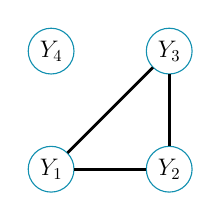
\begin{tikzpicture}
		\node[observed] (Z1) at (0*\edgeunit, 0*\edgeunit) {$Y_1$};
		\node[observed] (Z2) at (1*\edgeunit, 0*\edgeunit) {$Y_2$};
		\node[observed] (Z3) at (1*\edgeunit, 1*\edgeunit) {$Y_3$};
		\node[observed] (Z4) at (0*\edgeunit, 1*\edgeunit) {$Y_4$};
		\draw [line width=1pt] (Z1) -- (Z2); 
		\draw [line width=1pt] (Z1) -- (Z3); 
% 		\draw [line width=1pt] (Z1) -- (Z4); 
		\draw [line width=1pt] (Z2) -- (Z3); 
% 		\draw [line width=.1pt] (Z2) -- (Z4); 
% 		\draw [line width=1pt] (Z3) -- (Z4); 
		\end{tikzpicture}\\
		\emphase{$P\{(j, k) \in T | Y\}$}
	   \end{tabular}
	   &
	 \end{tabular}
   % \end{tabular}
   %\end{tabularx}
   \end{center}
\end{frame}
%====================================================================
%====================================================================

%====================================================================
%====================================================================
%====================================================================
%====================================================================


%====================================================================
%====================================================================
\section{Inference}
\begin{frame}
\begin{center}
\huge{\bleu{Inference}}
\end{center}
\end{frame}
\subsection{E step}
\begin{frame}{Direct EM algorithm ?}
\footnotesize 
\begin{itemize}
    \item \bleu{Complete likelihood :}

 \[ P(Y,Z,T) = \color{olive}P(T)\color{black}\times\color{blue}P(Z|T)\color{black}\times\color{orange}P(Y|Z)\]
 
\begin{align*}
 \log(P(Y,Z,T)) &= \sum_{k,l} \mathds{1}_{\{(k,l) \in T\}} (\color{olive}\log(\beta_{kl})\color{black} + \color{blue}\log(\psi_{kl}(Z)) \color{black})-\color{olive}\log(B)\color{black} \\
 &+\sum_k (\color{blue} \log(P(Z_k))\color{black} + \color{orange}\log(P(Y_k|Z_k))\color{black})
 \end{align*}
 
 \pause
 \item \bleu{Conditional expectation :}
\end{itemize}
\begin{align*}
    \mathds{E}_\theta[\log(P(Y,Z,T))|Y] =&\sum_{k,l} \mathds{P}((k,l) \in T|Y) \log(\beta_{kl}) + \mathds{E}[\mathds{1}_{\{(k,l) \in T\}}\emphase{\log(\psi_{kl}(Z)|Y)}]\\
& +\sum_k \emphase{\mathds{E}[\log(P(Z_k)) | Y]} + \mathds{E}[\log(P(Y_k|Z_k)) | Y]-\log(B)
\end{align*} 

\normalsize 
\end{frame}
%====================================================================
%====================================================================


\begin{frame}{Variational approximation}

 \begin{enumerate}
       \item The \emphase{{\fontfamily{qcr}\selectfont{PLNmodels}}} package approximates the distribution parameters $\hat{\Sigma}_Z,  \hat{\theta}$ \vspace{0.5cm}
       \item E step with : $ \mathds{E}_\theta[\log(P(Y,Z,T))|Y] \simeq \sum_{j,k} \emphase{P_{jk}} \log(\beta_{jk}\hat{\psi}_{jk}) -\log(B) + cste $,\\
       where      
$$\emphase{P_{jk}} =  \sum_{T:jk\in T} \prod_{jk \in T} \beta_{jk} \widehat{\psi}_{jk}/C \simeq   \mathds{P}(\{j,k\}\in T |Y) $$
 and $C$ is the normalizing constant: $C = \sum_T \prod_{j, k \in T} \beta_{jk} \widehat{\psi}_{jk}$.\\
   \end{enumerate}
   

\end{frame}

 %====================================================================
%====================================================================

\begin{frame}{Approximate conditional probability computation}
\footnotesize
\begin{exampleblock}{Kirchhoff's theorem (matrix tree, \cite{AiH89})}
For all $W=(a_{kl})_{k,l}$ a symmetric matrix, the corresponding Laplacian $Q(W)$ is defined as follows:
 \[Q_{uv}(W)=
 \begin{cases}
     -a_{uv} & 1\leq u<v \leq n\\
    \sum_{i=1}^n a_{vi} & 1\leq u=v \leq n.
\end{cases}
\]
Then for all $u$ et $v$:
    \[ |Q^*_{uv}(W)|=\sum_{T\in\mathcal{T}} \prod_{\{k,l\}\in E_T} a_{kl} \]
\end{exampleblock}
\begin{align*}
 P_{jk}&=\sum_{T:jk\in T} \prod_{jk \in T} \beta_{jk} \widehat{\psi}_{jk}/C\\
 &=\emphase{1- \frac{|Q^*_{uv}(\beta\Psi^{-kl})|}{|Q^*_{uv}(\beta\Psi)|}}
 \end{align*}
 
\end{frame}



%====================================================================
%====================================================================

\subsection{M step}
%\normalsize 
\begin{frame}{M step}
%\textbf{Goal} : optimization of weights $\beta_{kl}$.\\
%\vspace{1cm}
%\[\argmax_{\beta_{kl}} \left\{\sum_{j,k} \hat{P}_{jk}(\emphase{\log(\beta_{jk})} + \log(\hat{\psi}_{kl}) ) -\emphase{\log(B)} + cste \right\}\]
%
%  \vspace{1cm}
%  
% \[\text{With high combinatorial complexity of } B = \sum_{\emphase{T\in\mathcal{T}}} \prod_{k,l\in T} \beta_{kl}\]
% 
% \begin{center}
%     How to compute \Large{$\frac{\partial B}{\partial\beta_{kl}}$ }?
% \end{center}
%\end{frame}
% %====================================================================
%%====================================================================
%
% \begin{frame}{$\beta_{kl}$ update}
 \footnotesize 
 \begin{exampleblock}{A result from \cite{MixtTrees}}
Inverting a minor of the laplacien $Q$, we define M : 
\[\begin{cases}
    M_{uv} = [Q^{*-1}]_{uu} + [Q^{*-1}]_{vv} -2[Q^{*-1}]_{uv} & u,v < n\\
    M_{nv} =M_{vn} =[Q^{*-1}]_{vv} & v<n\\
     M_{vv} =0.
   \end{cases}\]
On peut montrer que :
\[ \frac{\partial|Q^*_{uv}(W)|}{\partial \beta_{kl}} = M_{kl} \times |Q^*_{uv}(W)|\]
\end{exampleblock}

\emphase{
   \large{\[\hat{\beta}_{kl}= \frac{P_{kl}}{M_{kl}}\]}
}
 \end{frame}
  %====================================================================
%====================================================================
\section{EMtree}
\subsection{}
\begin{frame}{EMtree algorithm}
\begin{description}
\normalsize
\item [Input: ] \hspace{0.35cm}Abundance data, covariates, offsets\vspace{0.2cm}

\item [1rst step: ] \hspace{0.3cm} \emphase{fit PLN model} $\Rightarrow$  $\hat{\theta}$, $\hat{\Sigma}_Z$. \vspace{0.2cm}
\item [2nd step: ] \hspace{0.3cm} \emphase{update the $\beta_{jk}$} $\Rightarrow$ conditional probabilities for all edges.\\ \hspace{0.3cm} 
%\pause
\bigskip
\item [Thresholding: ] Select edges with probability above the probability of edges in a tree drawn uniformly (\emphase{$2/p$})\vspace{0.2cm}
\item [Resampling: ] \hspace{0.25cm}Strengthen the results: keep only edges selected in more than \emphase{$80\%$} of $S$ sub-samples (selection threshold).
\end{description} \bigskip

Available for download at \url{https://github.com/Rmomal/EMtree}
\begin{figure}
    \centering
    \includegraphics[width=0.6cm]{github.png}
\end{figure}
\end{frame}

%====================================================================
%====================================================================

\begin{frame}
\begin{center}
\huge{\bleu{Comparison with state-of-the-art approaches}}
\end{center}
\end{frame}
\subsection{Performance}
\begin{frame}{Evaluation strategy}
\bleu{Alternatives:}\\
 Two methods  on \bleu{transformed counts, no covariates (on residuals)}:\\
    \begin{itemize}
        \item \emphase{SpiecEasi} algorithm \citet{kurtz} 
        \item \emphase{gCoda} \citet{gcoda} 
    \end{itemize}
    
    One taking \bleu{raw counts and covariates}:\\
    \begin{itemize}
        \item \emphase{MInt} \citet{MInt} (uses PLN model)
    \end{itemize}\bigskip
\pause
\bleu{Simulation design:}\\
\begin{enumerate}
     \item Choose  \emphase{$G$} and define  \emphase{$\Sigma_G$} accordingly
     \item Sample count data \emphase{$Y$} from $\mathcal{P\ell N}(X,\Sigma_G)$ 
     \item Infer the network with \emphase{EMtree},  \emphase{SpiecEasi},  \emphase{gCoda}, and  \emphase{MInt} 
     \item Compare results with  presence/absence of edges (\emphase{FDR}, \emphase{AUC})
\end{enumerate}

\end{frame}

%====================================================================
%====================================================================

\subsection{Results}
\begin{frame}{Tested graphs}
    \begin{figure}
        \centering
        \includegraphics[width=\linewidth]{graphs}
    \end{figure}
\end{frame}
\begin{frame}{Difficulty level}
\tiny{$S=150$, selection threshold$ = 80\%$}
\begin{figure}
    \centering
       \includegraphics[width=12.5cm]{TPFNErdos.png}\\
       \vspace{1cm}
    \includegraphics[width=9cm]{times_EH.png}
\end{figure}
\end{frame}

\begin{frame}{Effect of S on EMtree}
 \begin{figure}
  \centering
   \includegraphics[width=7cm]{compareS.png}\\
  \includegraphics[width=10cm]{timesS.png}
\end{figure}
\end{frame}

\begin{frame}{Network density}
    \begin{figure}
        \centering
        \includegraphics[width=9cm]{varyDens.png}
    \end{figure}
\end{frame}
\begin{frame}{data dimension : 2/p density}
    \begin{figure}
        \centering
       \hspace*{-0.5cm}%
        \includegraphics[width=\paperwidth]{auc2p}
    \end{figure}
\end{frame}

\begin{frame}{Data dimension : 5/p density}
    \begin{figure}
        \centering
        \hspace*{-0.4cm}%
        \includegraphics[width=\paperwidth]{auc5p}
    \end{figure}
\end{frame}
\begin{frame}{Data dimension : scale-free structure}
    \begin{figure}
        \centering
        \hspace*{-0.4cm}%
        \includegraphics[width=11cm]{sfauc}
    \end{figure}
\end{frame}
%====================================================================
%====================================================================

\section{Application}
\subsection{Oak data}

%====================================================================
%====================================================================
\begin{frame}
\begin{center}
\huge{\bleu{Application}}
\end{center}
\end{frame}
\begin{frame}{Oak Mildew}
\begin{columns}
\begin{column}{5cm}
\begin{figure}[htp]
\centering
\includegraphics[scale=0.07]{EA.jpg}
\caption{\textit{Pathogen Erysiphe alphitoides (EA).}}
\end{figure}
\end{column}
\begin{column}{6cm}
\begin{figure}[htp]
\centering
\includegraphics[scale=0.1]{mildew.jpg}
\caption{Oak leaf with powdery mildew.}
\end{figure}
\end{column}
\end{columns}
\vspace{0.5cm}
Metabarcoding of oak tree leaves microbiome \citep{jakuch}.\\

\begin{itemize}
	\item 116 sample of 114 bacterial/fungal OTUs
	\item Different read depth for bacteria and fungi
	\item covariates: tree status (Tree); distance to ground (D1), to trunk (D2), to base of the branch (D3).
\end{itemize}
\end{frame}
%====================================================================
%====================================================================

\begin{frame}{Inferred networks}
Selection threshold$=90\%$

    \begin{figure}[htp]
\hspace*{-0.7cm}%
\includegraphics[width=13.5cm]{Oaknet_90_btw.png}
\end{figure}
\end{frame}

\begin{frame}{Comparison of densities}
    \begin{figure}[htp]
\centering
\includegraphics[width=7.5cm]{qetOak.png}
\end{figure}
\end{frame}

\begin{frame}{Comparison with results from \cite{jakuch}}
    \begin{figure}[htp]
\centering
\includegraphics[width=10cm]{propOTUS.png}
\end{figure}
\end{frame}

%-----------------------------
%---------------------------
\begin{frame}{Wrap-up}
\begin{description}
\item[Contributions:] 
\begin{itemize}
\item[]  
	\item Formal probabilistic model for network inference with \emphase{count data}
	\item Inclusion of \emphase{offsets} and \emphase{covariates}
	\item  Variational estimation algorithm which behaves well compared to recent approaches
	\item Package EMtree and article available (GitHub / arXiv)
\end{itemize}
\bigskip 
\item[Perspectives:]

\begin{itemize}
\item[] 
	\item Accounting for spatial structure (more ecological data)
	\item Simulation study under an other model
	\item Missing major actor (species or covariates) 
	%\item Network comparison
\end{itemize}
\end{description}
\end{frame}
%====================================================================
%====================================================================

%\begin{frame}{Acknowledgments}
%
%Special thanks :\\
%\begin{description}
%\item[Supervisors] Stéphane Robin, Christophe Ambroise
%\item[PLN team] Julien Chiquet (MIA-Paris), Mahendra Mariadassou (INRA Jouy)
%\item[Data] Corinne Vacher (INRA Bordeaux)
%\end{description}
%Contact :\\
%\begin{description}
%\item[email] raphaelle.momal@agroparistech.fr
%\item[Web]Rmomal.github.io\\
%\end{description}
%\begin{center}
%	\includegraphics[width=0.25\linewidth]{logo_inra.jpg}\hspace{0.1cm}
%	\includegraphics[width=0.25\linewidth]{agro.PNG}
%	\includegraphics[width=0.25\linewidth]{lmh.png}\hspace{0.1cm}
%	\includegraphics[width=0.15\linewidth]{upsud.jpg}
%    
%\end{center}
%
%\end{frame}
\appendix
\backupbegin



\begin{frame}[allowframebreaks]
\bibliographystyle{apalike}
{\tiny
    \bibliography{biblio3.bib}}
\frametitle{References}
%\bibliography{cellcite}
\end{frame}\backupend
%====================================================================
%====================================================================

\end{document}